\begin{ledgroupsized}[r]{120mm}%
\footnotesize%
\pstart%
\noindent\textbf{\"{U}berlieferung:}%
\pend%
\end{ledgroupsized}%
\begin{ledgroupsized}[r]{114mm}%
\footnotesize%
\pstart%
\parindent -6mm%
\makebox[6mm][l]{\textit{L}}%
Auszüge mit Bemerkungen aus einem verschollenen Manuskript von René Descartes:
LH~III~4, 3a Bl.~1.
1 Bl. 2\textsuperscript{o}. Insgesamt etwa \nicefrac{1}{2}~S., teils im unteren Viertel von Bl.~1~r\textsuperscript{o}, teils im unteren Viertel von Bl.~1v\textsuperscript{o}.
Bl.~1~r\textsuperscript{o} überliefert auch N.~76. % LH003_04_03a_001r_text1 = Remedia et vires medicamentorum
Der Rest von Bl.~1~v\textsuperscript{o} ist leer.
\newline%
Cc 2, Nr. 1323 A (tlw.)%
\pend%
%
\pstart%
\parindent -6mm%
\makebox[6mm][l]{\textit{E}}%
\cite{00120}\textsc{R.~Descartes}, \textit{{\OE}uvres}, hrsg. von \textsc{C.~Adam} und \textsc{P.~Tannery}, Bd.~XI, Paris 1909, S.~645f.
\pend%
\end{ledgroupsized}%
%
\vspace*{5mm}%
\begin{ledgroup}%
\footnotesize%
\pstart%
\noindent%
\footnotesize{%
\textbf{Datierungsgr\"{u}nde:}
Das vorliegende Stück findet sich auf demselben Textträger wie die von Leibniz eigenhändig datierten Auszüge N.~76. 
% LH003_04_03a_001r_text1 = Remedia et vires medicamentorum
Beide Texte folgen unmittelbar aufeinander und sind nur durch einen waagerechten Strich voneinander abgesetzt.
Die Datierung von N.~76 % LH003_04_03a_001r_text1 = Remedia et vires medicamentorum
wird demgemäß auch für das vorliegende Stück übernommen.%
}%
\pend%
\end{ledgroup}%
%
%
\vspace*{8mm}%
\pstart%
\normalsize%
\noindent%
% [1~r\textsuperscript{o}]
[1~r\textsuperscript{o}] \textso{De refractione.}\protect\index{Sachverzeichnis}{refractio}
Vitri cujus refractio est ut 7 ad $\sqrt{\displaystyle113}$.
Si diameter sit \textit{c}, crassitudo erit $\displaystyle\frac{1}{36}c$
vel circiter nempe \rule[-4mm]{0mm}{10mm}$\displaystyle-\frac{7}{2}c + \sqrt{\displaystyle\frac{49}{4}cc + \displaystyle\frac{49}{256}cc}$
et altitudo machinae ad eam poliendam est $4c$ et longitudo ad focum est $9c$ fere.
\pend%
%
\pstart%
Refractio\protect\index{Sachverzeichnis}{refractio} in vitro
\edtext{ex experimentis D. Beaune,\protect\index{Namensregister}{\textso{Beaune}, Florimond 1601-1652}}{\lemma{ex experimentis D. Beaune}\Cfootnote{Nicht nachgewiesen.}}
est ut 1181 ad 768 fere.
\pend%
%
\pstart%
Refractio\protect\index{Sachverzeichnis}{refractio} ex aere ad aquam minor est,
quam ex aere ad 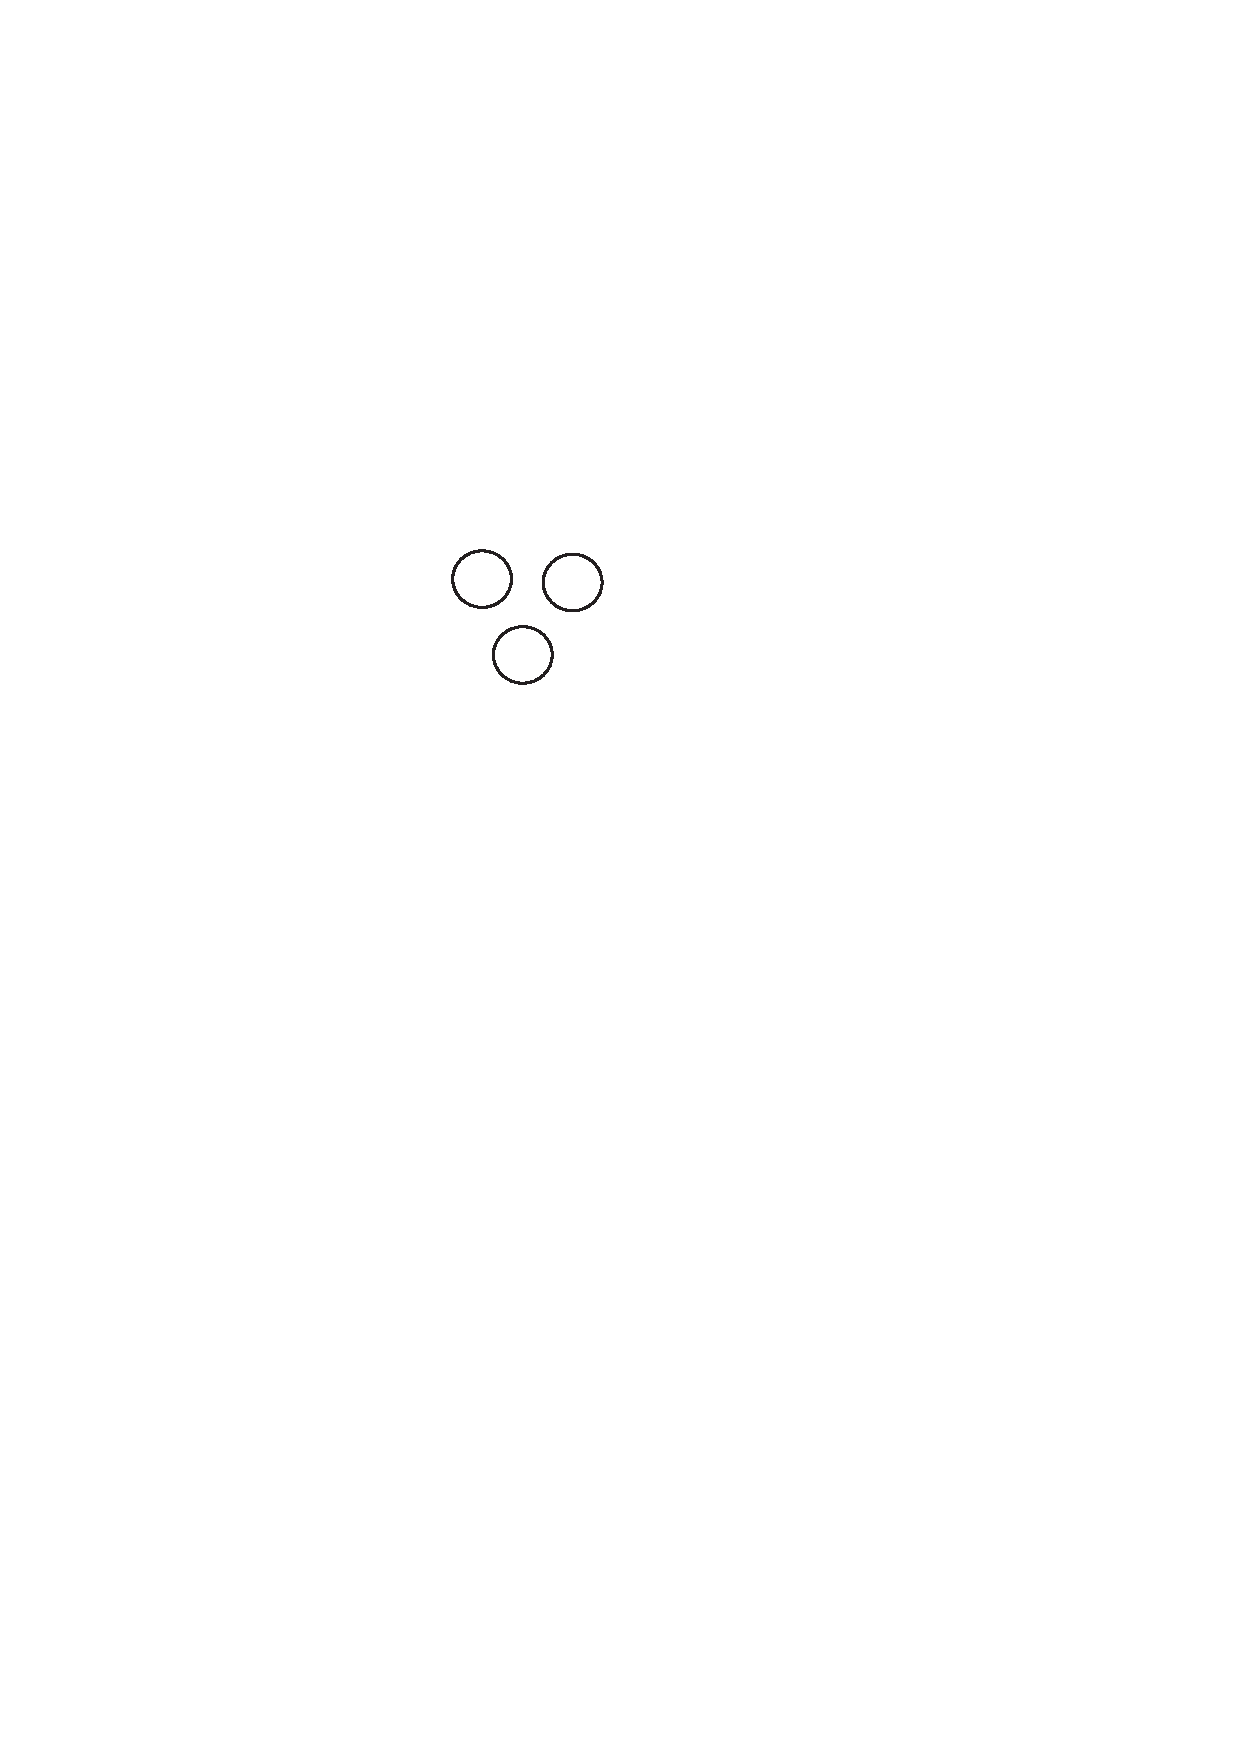
\includegraphics[width=0.022\textwidth]{images/oleum.pdf} 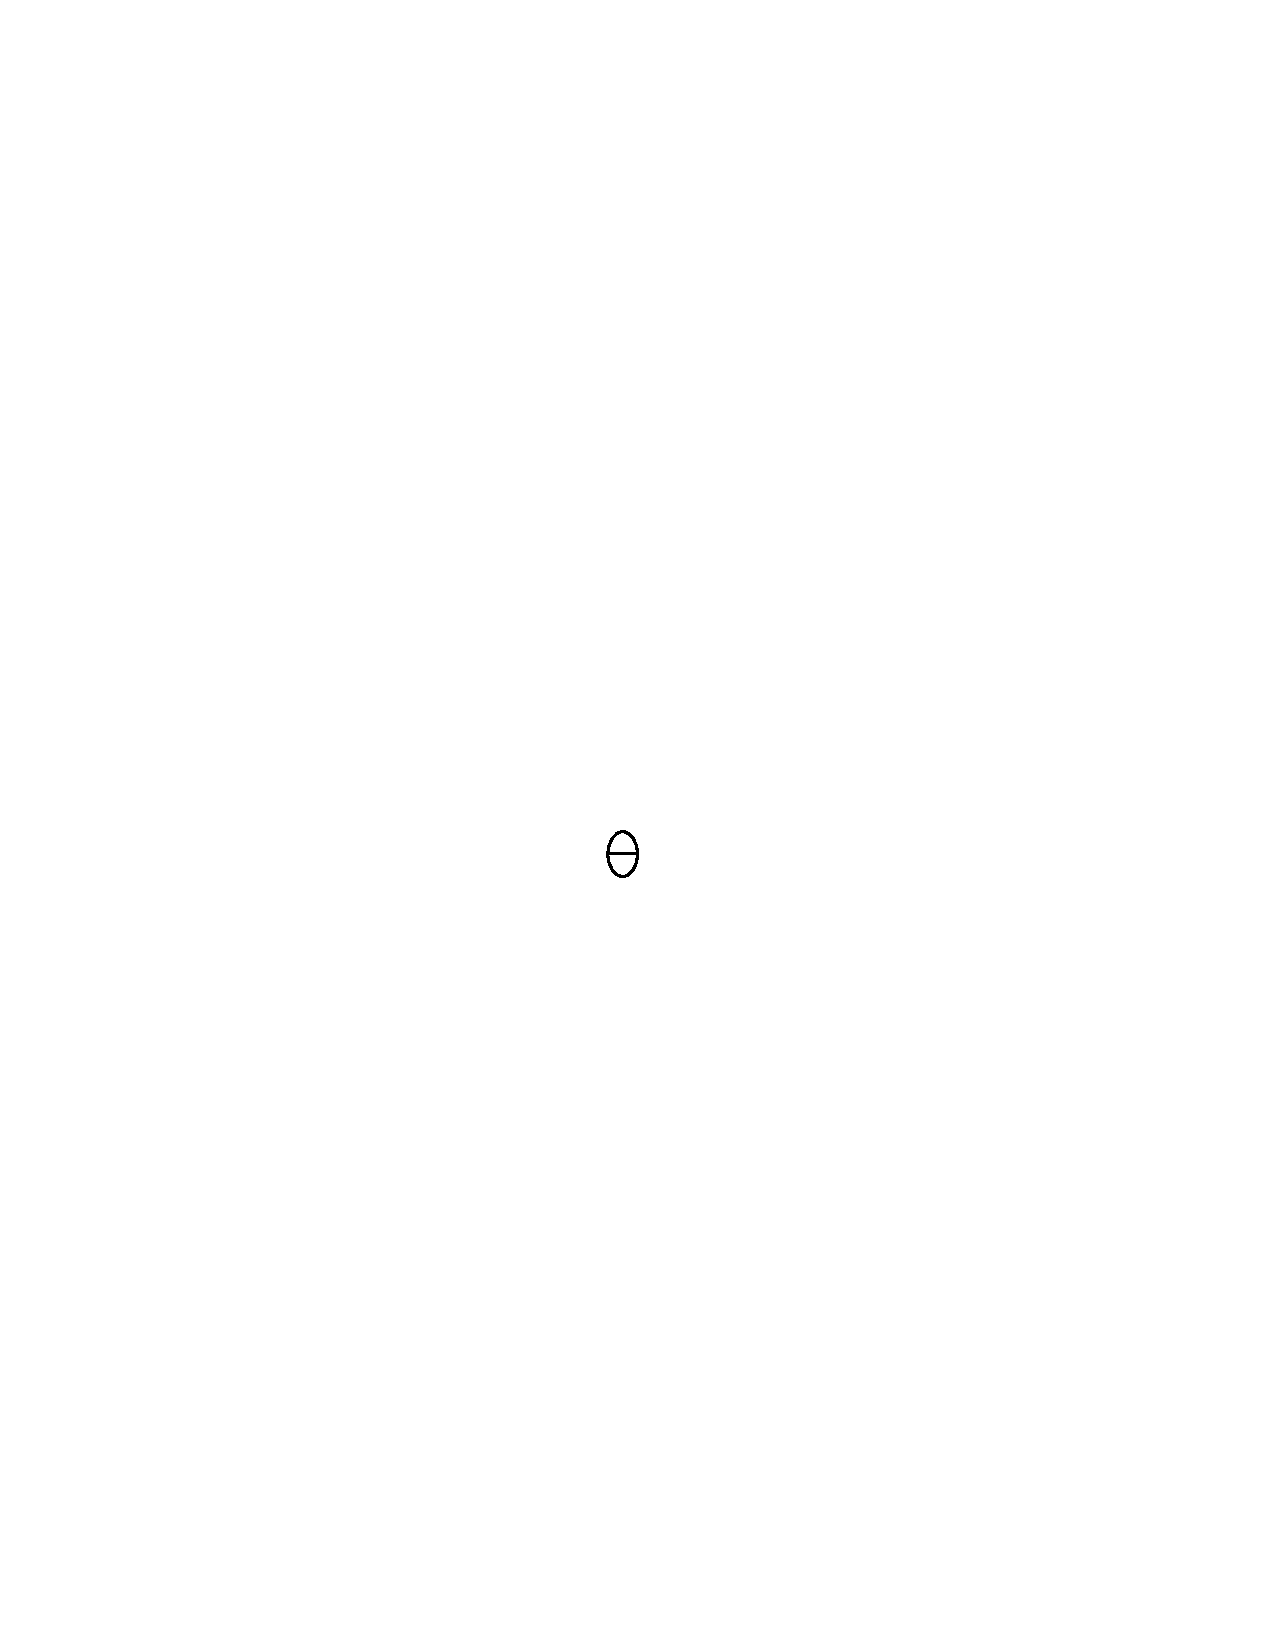
\includegraphics[width=0.016\textwidth]{images/sym-sal.pdf},
haec minor quam ad 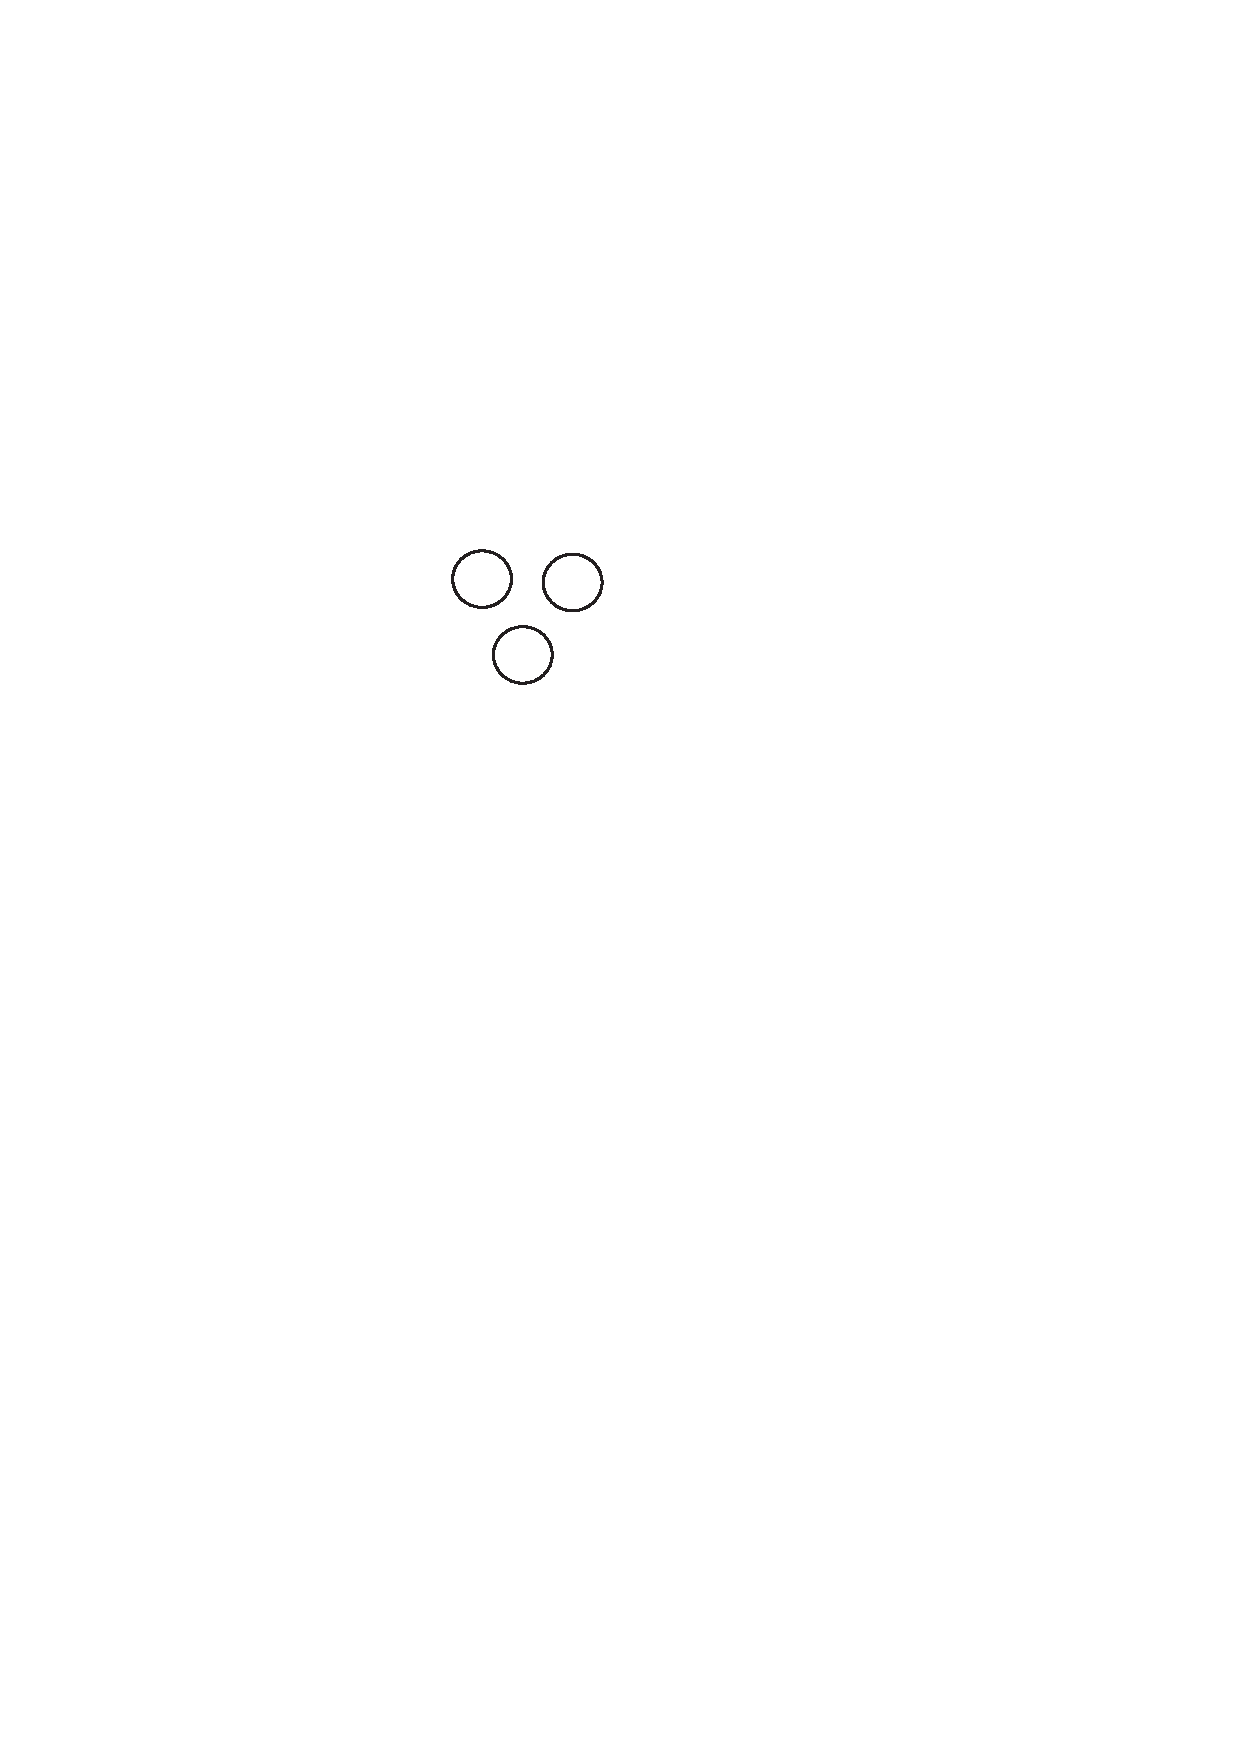
\includegraphics[width=0.022\textwidth]{images/oleum.pdf} Rosmarini\protect\index{Sachverzeichnis}{oleum rosmarini}
haec quam salviae,\protect\index{Sachverzeichnis}{oleum salviae}
haec quam thymi\protect\index{Sachverzeichnis}{oleum thymi}
haec quam caryophyllorum.\protect\index{Sachverzeichnis}{oleum caryophyllorum}
Refractio\protect\index{Sachverzeichnis}{refractio} autem quae fit in 
\includegraphics[width=0.022\textwidth]{images/oleum} caryo\pgrk{f}yllorum\protect\index{Sachverzeichnis}{oleum caryophyllorum}
circiter aequat illam quae fit in vitro solido.
\pend%
%
\pstart%
In 
\includegraphics[width=0.023\textwidth]{images/salpeter2.pdf}\protect\index{Sachverzeichnis}{aqua fortis} fere eadem est
quae in aqua communi, itemque in $\bigtriangledown$ salsa (+~miror~+) in calida vero minor (saepe expertum)%
\edtext{}{\lemma{}\Afootnote{\textit{Am Rand:} \Denarius\vspace{-4mm}}}
quam in frigida.
\pend%
%
\count\Bfootins=1200
\count\Cfootins=1200
\count\Afootins=1200
\pstart%
In spiritu vini\protect\index{Sachverzeichnis}{spiritus vini} multo major
\edtext{occurrit quam}{\lemma{}\Bfootnote{occurrit\ \textbar\ (+~miror~+) \textit{gestr.}\ \textbar\ quam \textit{ L}}}
in aqua communi, sed repetenda
\edtext{experientia.
[1~v\textsuperscript{o}]%
\newline%
\hspace*{7,5mm}%
Vitellio\protect\index{Namensregister}{\textso{Witelo} (Vitellio), um 1237-um 1280/90}%
}{\lemma{experientia.}\Bfootnote{\textit{(1)} \lbrack+~Si haec ita sunt, sequitur \textit{(2)} Vitellio \textit{ L}%
\quad\quad\quad
10
\
50 \textit{(1)} 20 \textit{(2)} 30 \textit{ L}
\quad\quad\quad
11
\
60 \textit{(1)} 24,30 \textit{(2)} 34,30 \textit{ L}
\quad\quad\quad
17f.
\
incidentiae \textbar\ incidentiae \textit{streicht Hrsg.} \textbar\ existente \textit{L}%
}}%
\edtext{ sic numerat angulos refractos[:]\protect\index{Sachverzeichnis}{angulus refractus}%
}{\lemma{Vitellio [...] refractos}\Cfootnote{\cite{01155}\textsc{Witelo}, \textit{Opticae libri decem}, Basel 1572, S.~412.
Die bei Witelo anzutreffenden Werte unterscheiden sich mehrfach von den in der Tabelle angegebenen.
Ferner weicht die Tabelle mit den Werten 12,5 und 7,5 vom Sexagesimalsystem ab.}}
\pend%
\vspace*{1.5em}% PR: Rein provisorisch !!!
%
\pstart%
\noindent
%\begin{tabular}{|p{1.7 cm}|p{2.4 cm}|p{2.4 cm}|p{2.4 cm}|p{2.4 cm}|}%
%\hline%
%anguli&refracti ab&refracti ab&refracti ab&refracti ab\\%
%incidentiae&aere ad aquam&aqua ad vitrum&aqua ad aerem&aere ad vitrum\\%
%\hline%
%10&7,45&9,30&12,5&7,5\\%
%20&15,30&18,30&24,30&13,30\\%
%\hline%
%30&22,30&27&37,30&19,30\\%
%40&29&35&31&25\\%
%\hline%
%50&30&42&65&30\\%
%60&34,30&30&79,30&34,30\\%
%\hline%
%70&28,30&49&94,30&38,30\\%
%80&42&30&110&42\\%
%\hline%
%\end{tabular}%
%
%\centering
\begin{tabular}{|l|l|l|l|l|}%
\hline%
anguli&refracti ab&refracti ab&refracti ab&refracti ab\\%
\protect{incidentiae\renewcommand*{\raggedleftmarginnote}{} \reversemarginpar\marginnote{\scriptsize\hspace{47.8mm}5}}
&aere ad aquam&aqua ad vitrum&aqua ad aerem&aere ad vitrum\\%
\hline%
10&7,45&9,30&12,5&7,5\\%
20&15,30&18,30&24,30&13,30\\%
\hline%
30&22,30&27&37,30&19,30\\%
40&29&35&31&25\\%
\hline%
{50\renewcommand*{\raggedleftmarginnote}{} \reversemarginpar\marginnote{\scriptsize\hspace{46mm}10}}
&30&42&65&30\\%
60&34,30&30&79,30&34,30\\%
\hline%
70&28,30&49&94,30&38,30\\%
80&42&30&110&42\\%
\hline%
\end{tabular}
\pend%
\vspace*{1.5em}% PR: Rein provisorisch !!!
\pstart%
Cum \setline{14}facit refractum ab aqua ad aerem ex complemento ejus quod est ab aere ad aquam,
necessario errat, nam cum refractio\protect\index{Sachverzeichnis}{refractio} in ingressu et egressu sit aequalis,
si angulo incidentiae\protect\index{Sachverzeichnis}{angulus incidentiae} existente 30 graduum sit refractus 22,30;
erit contra ab aqua ad aerem angulo incidentiae existente 22,30;
refractus 30 graduum ac per consequens angulo
incidentiae\protect\index{Sachverzeichnis}{angulus incidentiae} existente
30 grad. refractus erit amplius quam 37,30.
Sed totae hae tabulae sunt falsae.%
\pend%
\count\Bfootins=1500
\count\Cfootins=1500
\count\Afootins=1500
%%%%  PR: Hier endet das Stück.